\documentclass[11pt]{amsart}

%-----------------Preprocessed Packages----------------%
\usepackage{geometry}                % See geometry.pdf to learn the layout options. There are lots.
\geometry{letterpaper}
%\geometry{landscape}                % Activate for for rotated page geometry
%\usepackage[parfill]{parskip}      % Activate to begin paragraphs with an empty line rather than an indent
\usepackage{graphicx}
\usepackage{amssymb}
\usepackage{epstopdf}
\DeclareGraphicsRule{.tif}{png}{.png}{`convert #1 `dirname #1`/`basename #1 .tif`.png}
%-----------------------------------------------------------------%

%-------------------Landscape Package------------------%
\usepackage{pdflscape}
%-----------------------------------------------------------------%

%---------------------Listings Package--------------------%
\usepackage{listings}
\usepackage{color}
\definecolor{mygreen}{rgb}{0,0.6,0}
\definecolor{mygray}{rgb}{0.5,0.5,0.5}
\definecolor{mymauve}{rgb}{0.58,0,0.82}
\lstset{ %
  backgroundcolor=\color{white},   % choose the background color; you must add \usepackage{color} or \usepackage{xcolor}
  basicstyle=\footnotesize,        % the size of the fonts that are used for the code
  breakatwhitespace=flase,         % sets if automatic breaks should only happen at whitespace
  breaklines=false,                 % sets automatic line breaking
  captionpos=b,                    % sets the caption-position to bottom
  commentstyle=\color{mygreen},    % comment style
  deletekeywords={...},            % if you want to delete keywords from the given language
  escapeinside={\%*}{*)},          % if you want to add LaTeX within your code
  extendedchars=true,              % lets you use non-ASCII characters; for 8-bits encodings only, does not work with UTF-8
  frame=single,	                   % adds a frame around the code
  keepspaces=true,                 % keeps spaces in text, useful for keeping indentation of code (possibly needs columns=flexible)
  keywordstyle=\color{blue},       % keyword style
  language=Octave,                 % the language of the code
  otherkeywords={*,...},           % if you want to add more keywords to the set
  numbers=left,                    % where to put the line-numbers; possible values are (none, left, right)
  numbersep=5pt,                   % how far the line-numbers are from the code
  numberstyle=\tiny\color{mygray}, % the style that is used for the line-numbers
  rulecolor=\color{black},         % if not set, the frame-color may be changed on line-breaks within not-black text (e.g. comments (green here))
  showspaces=false,                % show spaces everywhere adding particular underscores; it overrides 'showstringspaces'
  showstringspaces=false,          % underline spaces within strings only
  showtabs=false,                  % show tabs within strings adding particular underscores
  stepnumber=2,                    % the step between two line-numbers. If it's 1, each line will be numbered
  stringstyle=\color{mymauve},     % string literal style
  tabsize=2,	                   % sets default tabsize to 2 spaces
  title=\lstname                   % show the filename of files included with \lstinputlisting; also try caption instead of title
}
%-----------------------------------------------------------------%

%---------------------Caption Package--------------------%
\usepackage{caption}
\DeclareCaptionFont{white}{ \color{white} }
\DeclareCaptionFormat{listing}{
  \colorbox[cmyk]{0.43, 0.35, 0.35,0.01 }{
    \parbox{1.25\textwidth}{\hspace{15pt}#1#2#3}
  }
}
\captionsetup[lstlisting]{ format=listing, labelfont=white, textfont=white, singlelinecheck=false, margin=0pt, font={bf,footnotesize} }
%-----------------------------------------------------------------%

\usepackage{csvsimple}

%----------------------Title Information---------------------%
\title{Numerical Methods\\ECSE 543 - Assignment 1}
\author{Mido Assran - 260505216}
\date{\today}                                           % Activate to display a given date or no date
%-----------------------------------------------------------------%



%----------------------BEGIN DOCUMENT---------------------%
\begin{document}
\maketitle


%----------------------BEGIN Question 1---------------------%
\section*{Question 1}

\subsection*{Part a}
The Choleski implementation is provided in \textbf{Listing \ref{lstng:choleski}}.

\subsubsection*{Code structure} To maintain portability and modularity of the code, object oriented principles were used for the software architecture. The choleski implementation is included in the \textit{CholeskiDecomposition()} class. The \textit{solve(A, b)} method solves the linear system of equations shown in equation (\ref{eq:linear_system}) by performing choleski elimination. 
\begin{equation}\label{eq:linear_system}
Ax = b
\end{equation}
The method accepts the matrix $A$, and the vector $b$ (both of which will eventually be overwritten by the algorithm in order to conserve memory resources), and returns the vector $x$ corresponding to the solution of equation (\ref{eq:linear_system}). The algorithm works in two stages. The first stage performs a choleski factorization of $A$ into $L L^T$ (overwriting the lower triangular part of $A$ by $L$), while simultaneously solving lower triangular system $Ly = b$ using forward substitution (overwriting $b$ with the solution $y$). At the end of this stage, the program state now contains $L$ in the lower triangular half of the matrix $A$, and the solution to $Ly=b$ in the vector $b$. In the second stage the program solves the system $L^Tx = y$ using backwards substitution (overwriting $y$ again with the solution $x$), where $y$ is the solution to the system solved in the first stage. The program subsequently returns the vector $x$, which is the solution to equation (\ref{eq:linear_system}).


\subsection*{Part b}
For testing purposes, it was necessary to create a symmetric positive definite matrix. Such a matrix was created using the \textit{generate\_positive\_semidef(order, seed)} method contained in the utils file in \textbf{Listing \ref{lstng:utils}}. Given an order (the dimension of the desired matrix), and an integer valued seed (used to seed the random number generator with a standard normal distribution), the function creates a random matrix, multiplies it by its transpose, and returns the result. The mathematical proof for why such a matrix is symmetric positive definite is well established. Whether or not the matrix is singular in this semidefinite method is important, and this is being checked by comparing the rank of the matrix to its order. If the rank of the matrix is not equal to the order of the matrix, then the matrix is singular and a warning is printed to the console. Note that this check still does not prevent the matrix from having a poor condition number. 


\subsection*{Part c}
The testing of the choleski implementation was conducted using the code provided under the \textit{main()} method in \textbf{Listing \ref{lstng:choleski}} lines $90 - 111$. The vector $x^*$, corresponding to the variable $x$ in equation (\ref{eq:linear_system}), is randomly generated with a standard normal distribution, and subsequently multiplied by the matrix $A$ in order to generate a third vector $b$  (i.e $b = A \cdot x^*$). The matrix $A$ and the vector $b$ are subsequently supplied to the solver, and the result is compared with the vector $x^*$ that was originally used to create $b$. A sample of the console output is provided in Figure \ref{fig:choleski_testing} - the matrix $A$ is of order $10$ in this example. The error in the produced result is quantified using the 2-norm: $$error = ||solve(A, b) - x^*||_2$$ As is seen in the console output, the error is only $2 \cdot 10^{-13}$, indeed the algorithm is producing the correct result. A possible reason for such a value of the error could be the roundoff error related to the condition of the randomly generated matrices.
\begin{center}
	\begin{figure}[h]
		\caption{Choleski Elimination Testing}
		\vspace*{1em}
		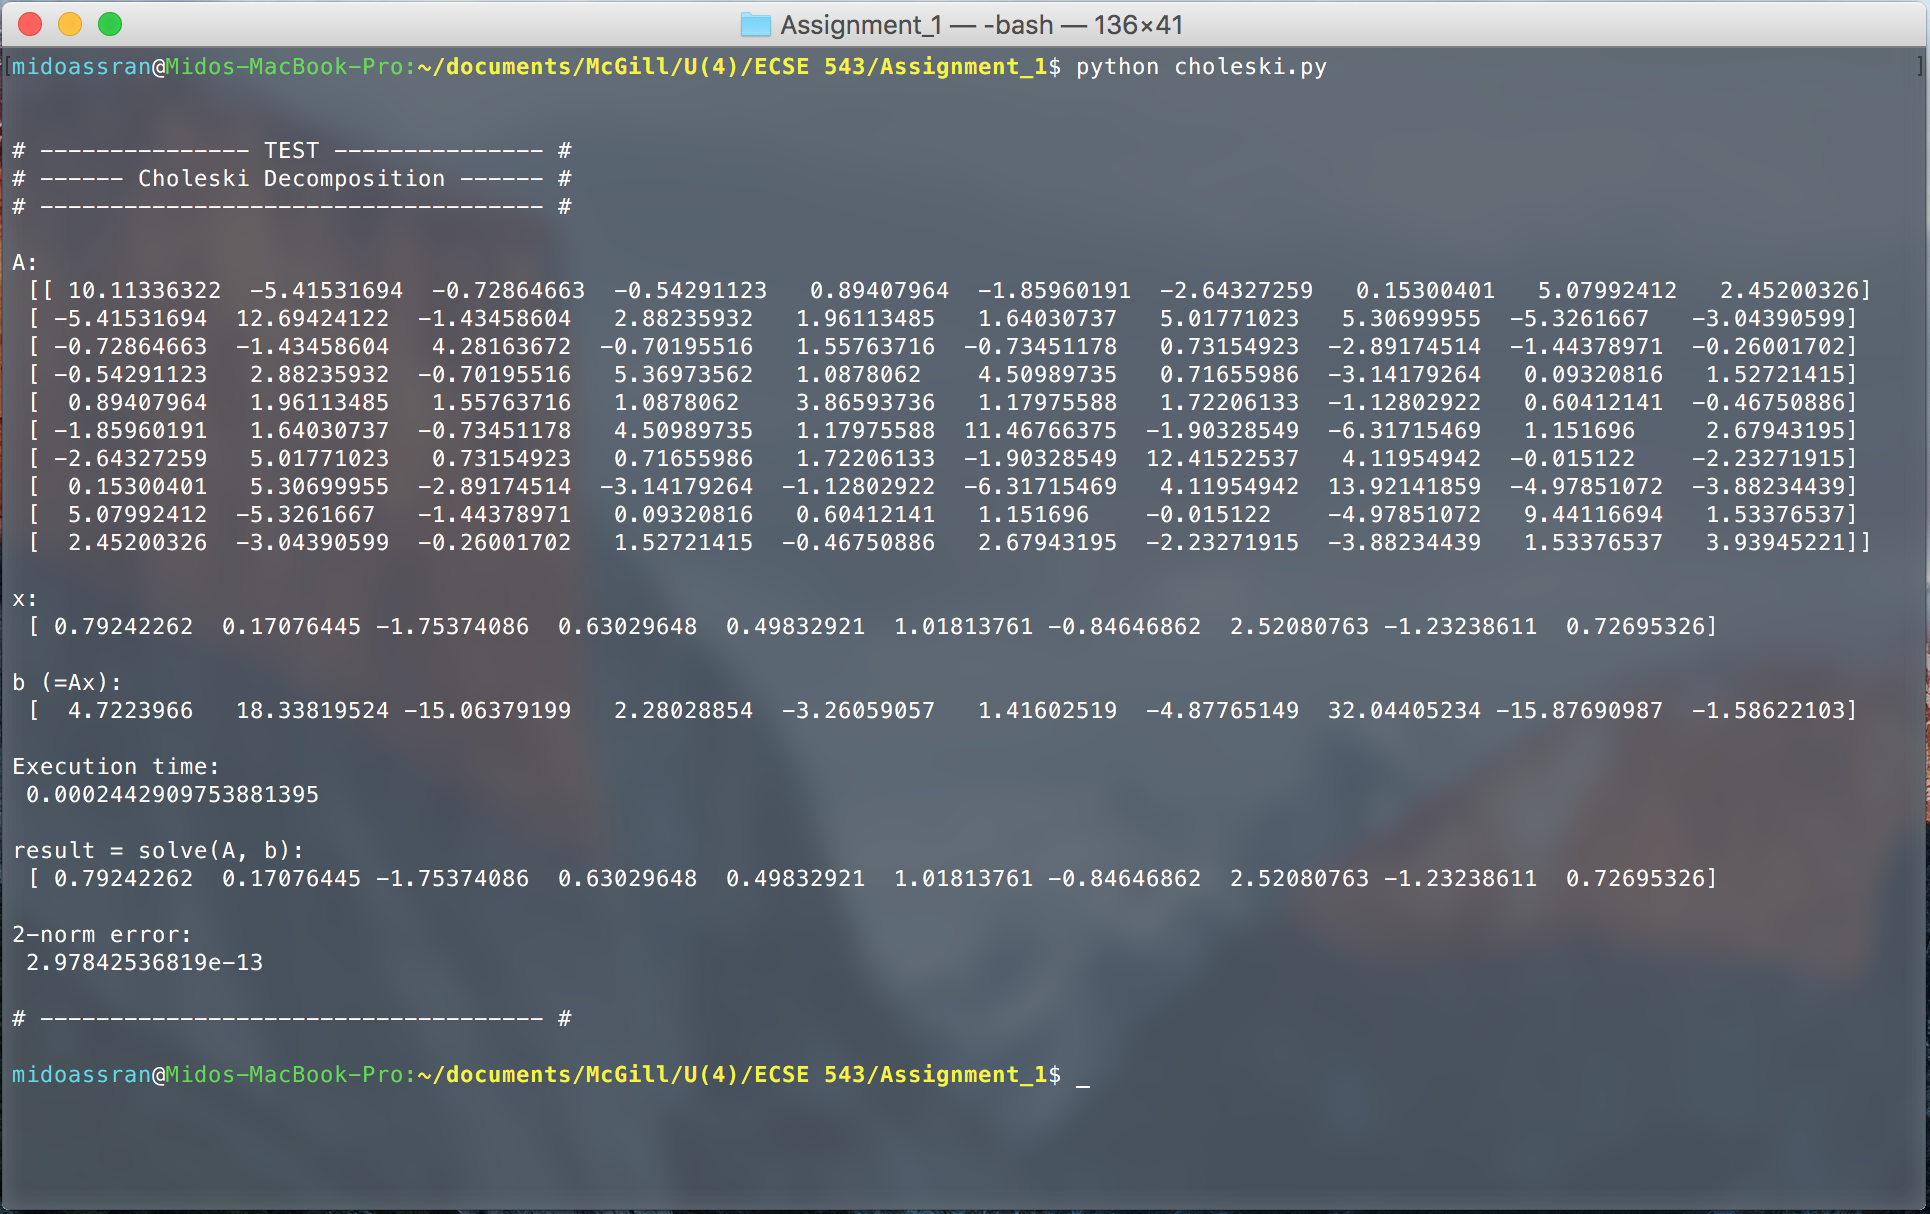
\includegraphics[width=\textwidth]{assets/choleski_testing.png}\label{fig:choleski_testing}
	\end{figure}
\end{center}


\subsection*{Part d}
A program used to solved tor the node voltages in a linear resistive network is provided in \textbf{Listing \ref{lstng:lrn_solver}}. The \textit{LinearResistiveNetworkSolver()} class is initialized with a filename from which to read the circuit description. The program, in the intializer, reads a list of network branches $(J_k, R_k, E_k)$ and a reduced incidence matrix from a CSV file. The format of the file is as follows: a set of rows (corresponding to each branch in the network), containing the comma separated branch current, resistance, and voltage in that respective order. Then a period is printed on a new line, to signify the end of the network data. The subsequent comma separated rows denote the incidence matrix, where each row corresponds to a node, and each column to a branch. An entry of $-1$ is used to indicate current entering a branch, $1$ is used to indicate current leaving a branch, and $0$ is used to indicate that the branch does not interact directly with the given node. The program reads the data in the file sequentially (i.e first the rows of the branch data are read, and then the rows of the incidence matrix are read). Once the data is read, the program subsequently generates a linear system of equations using the aforementioned data, and solves the system via choleski elimination.

\subsection*{Test Circuits} Test circuit CSV descriptions (used to test the program), and their equivalent circuit diagrams and corresponding console outputs are shown below. In each case, the console output was consistent with the analytical results obtained by hand.\\[0.1in]
\pagebreak

%---------------- Circuit 1 ----------------%
\begin{minipage}{\textwidth}
    \textit{Test Circuit 1}\\
    \noindent\rule[0.5ex]{\linewidth}{0.5pt}
\end{minipage}
\begin{minipage}{0.3\textwidth}
    \csvloop{file={../data/test_c1.csv},
    		no head,
                 before reading=\textbf{test\_c1.csv}\\[0.05in],
    		late after line={{,}\ }, 
    		late after line=\\ }
\end{minipage}
\begin{minipage}{0.7\textwidth}
	\begin{center}
		\vspace{1em}
        		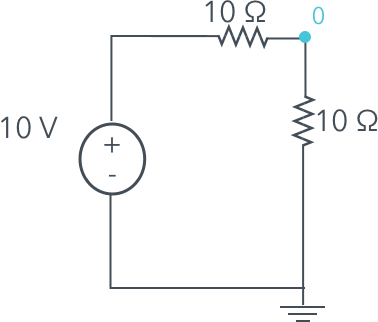
\includegraphics[width=0.6\textwidth]{assets/sk_test_c1.png}
	\end{center}
\end{minipage}
\begin{minipage}{\textwidth}
	\vspace{2em}
	\centering
	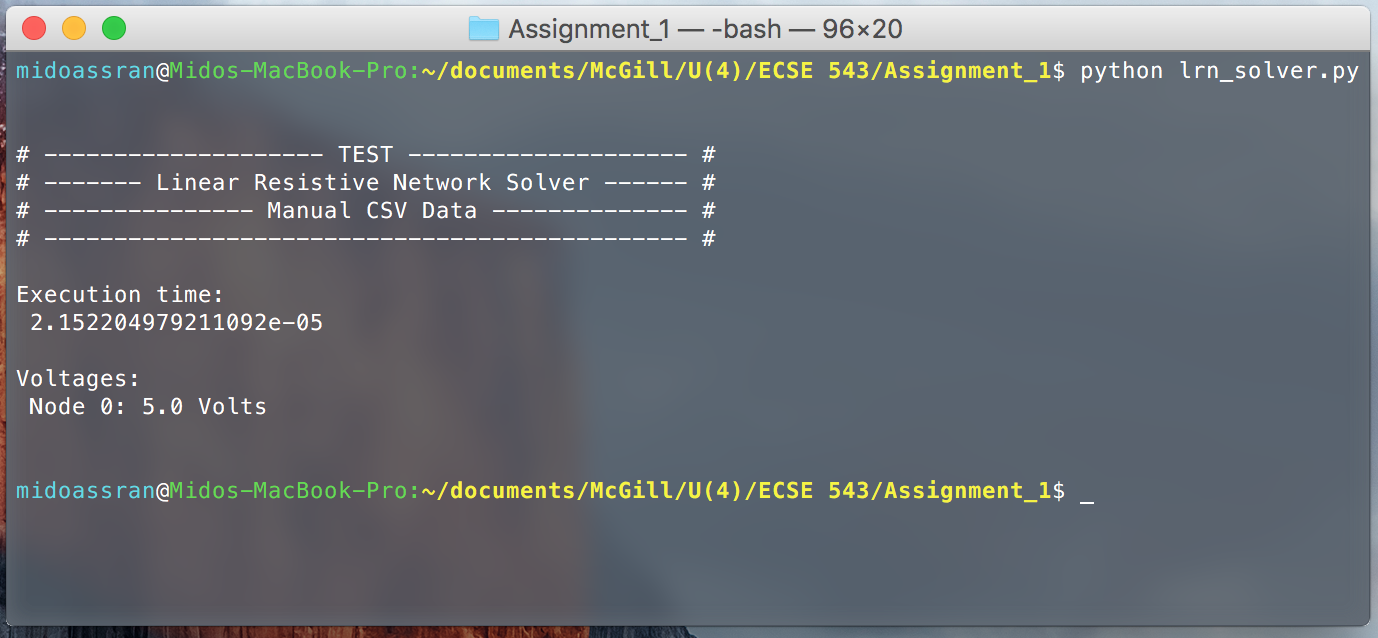
\includegraphics[width=\textwidth]{assets/test_c1.png}
\end{minipage}
\pagebreak
%---------------------------------------------%

%---------------- Circuit 2 ----------------%
\begin{minipage}{\textwidth}
    \textit{Test Circuit 2}\\
    \noindent\rule[0.5ex]{\linewidth}{0.5pt}
\end{minipage}
\begin{minipage}{0.3\textwidth}
    \csvloop{file={../data/test_c2.csv},
    		no head,
                 before reading=\textbf{test\_c2.csv}\\[0.05in],
    		late after line={{,}\ }, 
    		late after line=\\ }
\end{minipage}
\begin{minipage}{0.7\textwidth}
	\begin{center}
		\vspace{2em}
        		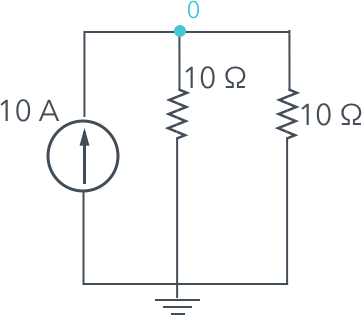
\includegraphics[width=0.55\textwidth]{assets/sk_test_c2.png}
	\end{center}
\end{minipage}
\begin{minipage}{\textwidth}
	\vspace{2em}
	\centering
	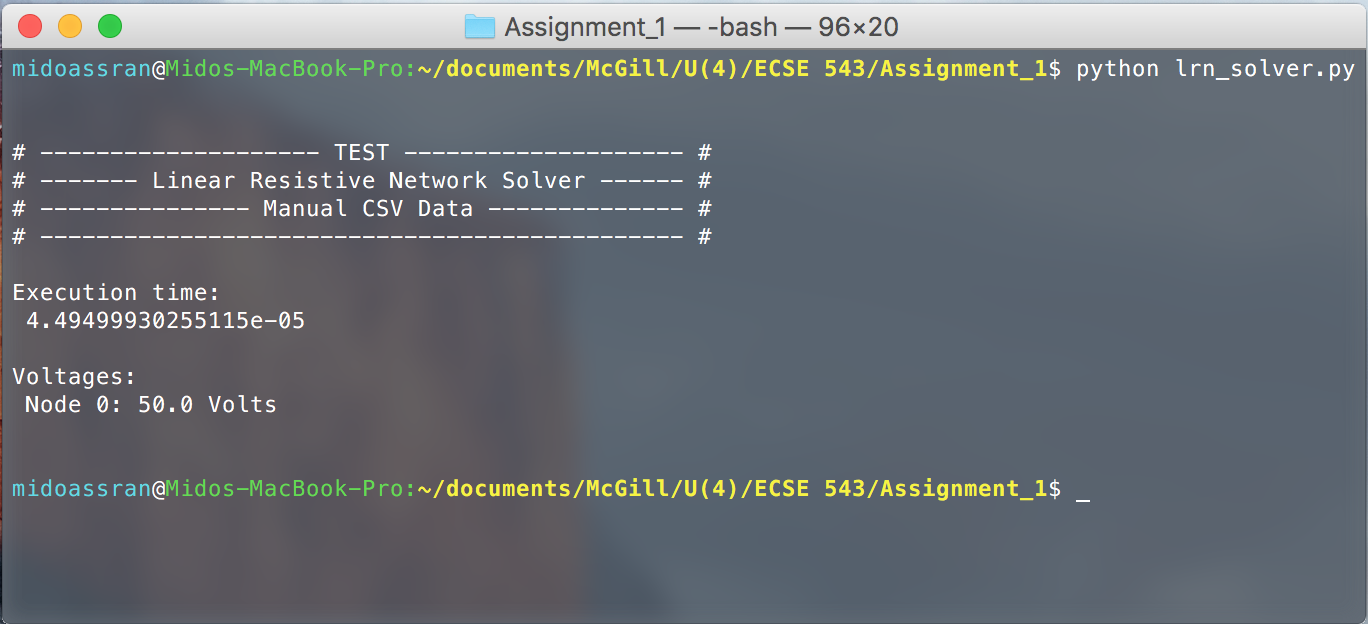
\includegraphics[width=\textwidth]{assets/test_c2.png}
\end{minipage}
\pagebreak
%---------------------------------------------%

%---------------- Circuit 3 ----------------%
\begin{minipage}{\textwidth}
    \textit{Test Circuit 3}\\
    \noindent\rule[0.5ex]{\linewidth}{0.5pt}
\end{minipage}
\begin{minipage}{0.3\textwidth}
    \csvloop{file={../data/test_c3.csv},
    		no head,
                 before reading=\textbf{test\_c3.csv}\\[0.05in],
    		late after line={{,}\ }, 
    		late after line=\\ }
\end{minipage}
\begin{minipage}{0.7\textwidth}
	\begin{center}
		\vspace{2em}
        		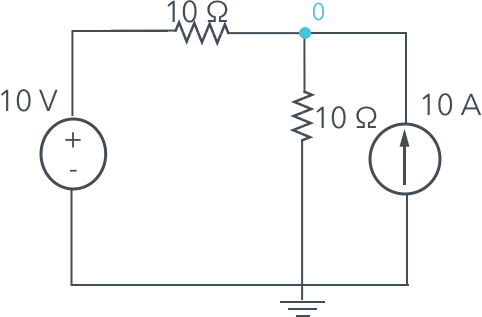
\includegraphics[width=0.8\textwidth]{assets/sk_test_c3.png}
	\end{center}
\end{minipage}
\begin{minipage}{\textwidth}
	\vspace{2em}
	\centering
	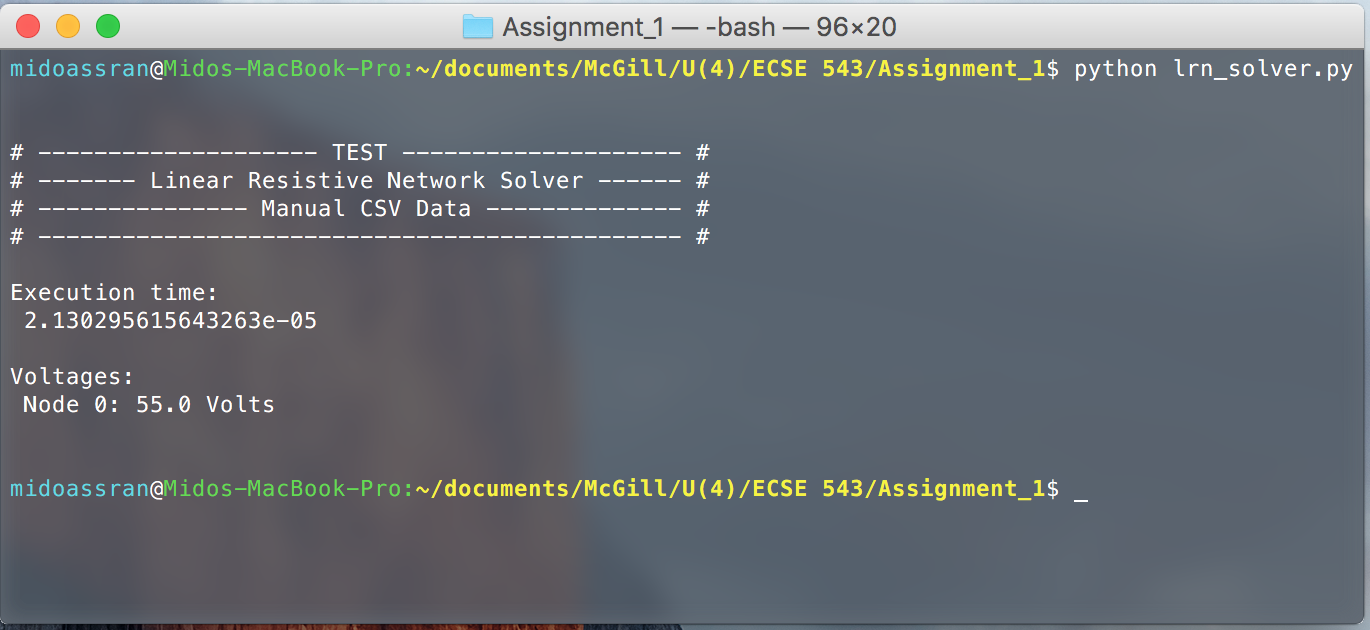
\includegraphics[width=\textwidth]{assets/test_c3.png}
\end{minipage}
\pagebreak
%---------------------------------------------%

%---------------- Circuit 4 ----------------%
\begin{minipage}{\textwidth}
    \textit{Test Circuit 4}\\
    \noindent\rule[0.5ex]{\linewidth}{0.5pt}
\end{minipage}
\begin{minipage}{0.25\textwidth}
    \csvloop{file={../data/test_c5.csv},
    		  no head,
                   before reading=\textbf{test\_c4.csv}\\[0.05in],
    		  late after line={{,}\ }, 
    		  late after line=\\ }
\end{minipage}
\begin{minipage}{0.8\textwidth}
	\begin{center}
		\vspace{2em}
        		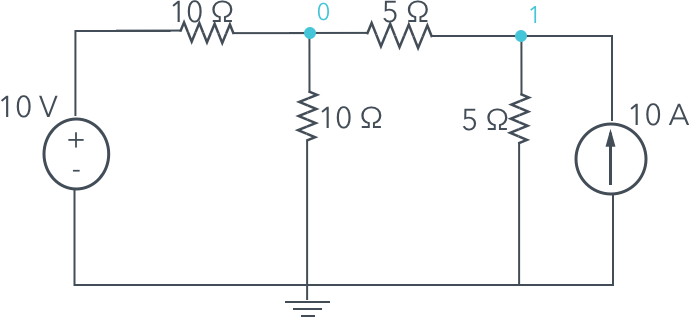
\includegraphics[width=\textwidth]{assets/sk_test_c4.png}
	\end{center}
\end{minipage}
\begin{minipage}{\textwidth}
	\vspace{2em}
	\centering
	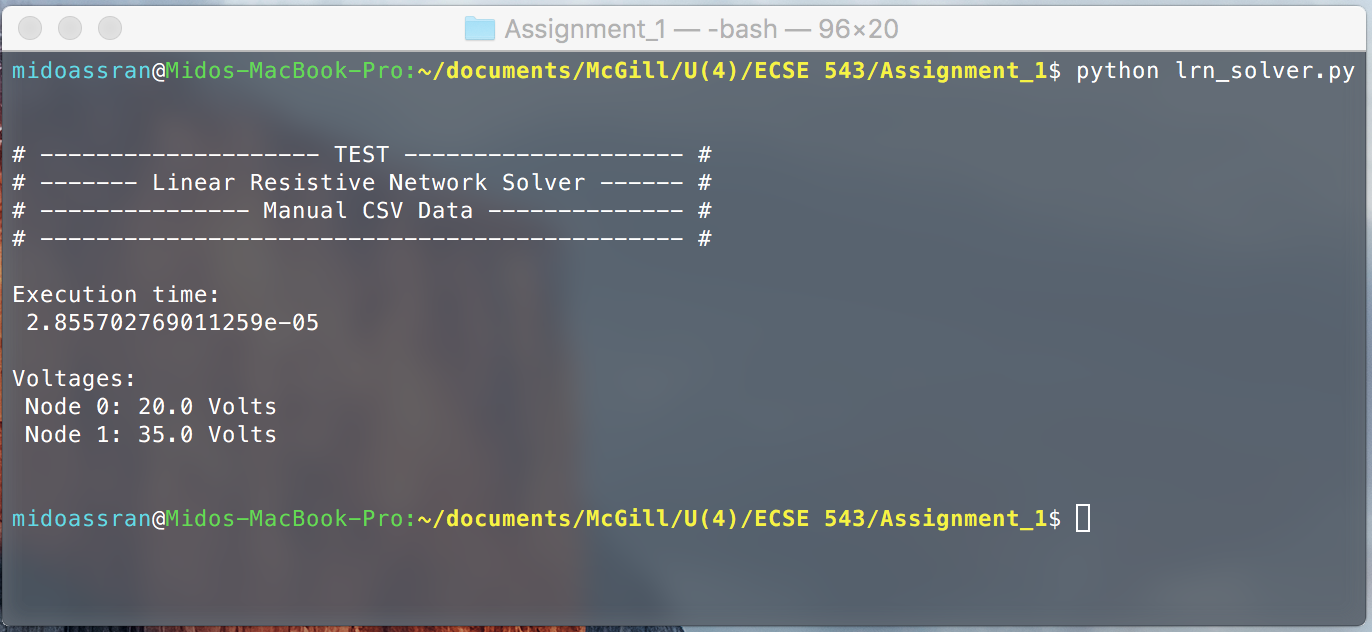
\includegraphics[width=\textwidth]{assets/test_c4.png}\\
\end{minipage}
\pagebreak
%---------------------------------------------%

%---------------- Circuit 5 ----------------%
\begin{minipage}{\textwidth}
    \textit{Test Circuit 5}\\
    \noindent\rule[0.5ex]{\linewidth}{0.5pt}
\end{minipage}
\begin{minipage}{0.3\textwidth}
    \csvloop{file={../data/test_c5.csv},
    		 no head,
                  before reading=\textbf{test\_c5.csv}\\[0.05in],
    		 late after line={{,}\ }, 
    		 late after line=\\ }
\end{minipage}
\begin{minipage}{0.7\textwidth}
	\begin{center}
		\vspace{2em}
        		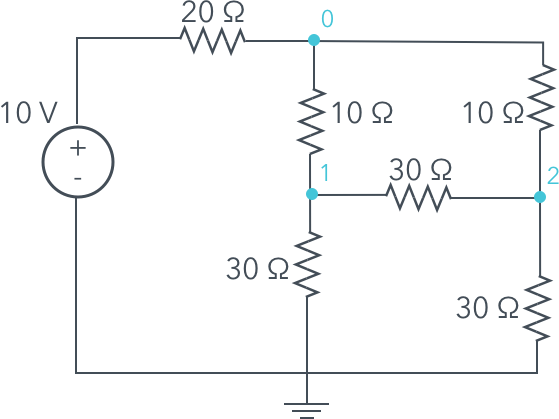
\includegraphics[width=\textwidth]{assets/sk_test_c5.png}
	\end{center}
\end{minipage}
\begin{minipage}{\textwidth}
	\vspace{2em}
	\centering
	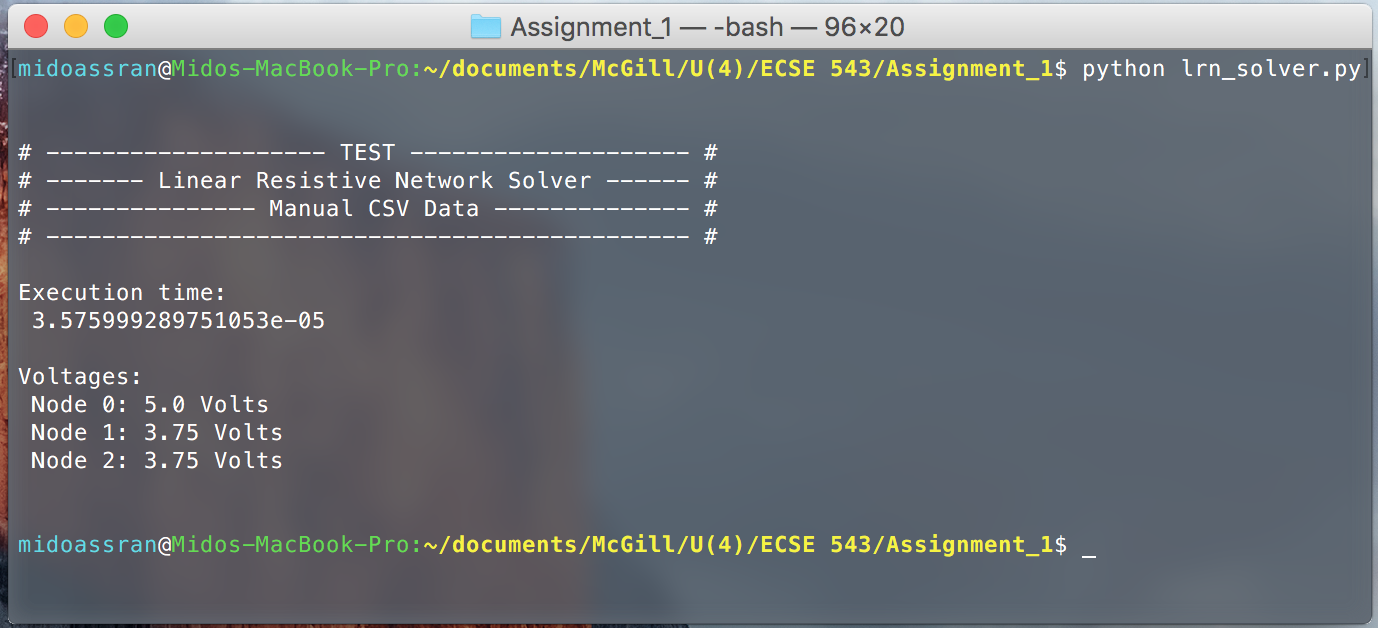
\includegraphics[width=\textwidth]{assets/test_c5.png}\\
\end{minipage}
\pagebreak
%---------------------------------------------%

\section*{Question 2}

\subsection*{Part a} To find the resistance across two diagonally opposing corners of a linear resistive N by N finite different mesh, the linear resistive network solver, provided in \textbf{Listing \ref{lstng:lrn_solver}}, was used. This is the same program that was used in Question 1. The static method \textit{create\_lrn\_mesh\_data(N, fname)} accepts an integer, $N$, denoting the size of the mesh, and a filename, to which a CSV description of the created mesh should be saved. It should be noted that this method also includes in the circuit description a test source placed across the diagonal of the mesh. This test source has a voltage of $1V$, and an output resistance of $1 \Omega$. The \textit{main()} method in \textbf{Listing \ref{lstng:lrn_solver}} - lines 166-177 - calls the appropriate methods to create the resistive finite difference mesh, and subsequently solve for all the node voltages. Once all the node voltages are known, the voltage difference between the two corners of the mesh is used to construct a simple voltage division equation that is used to solver for the equivalent resistance of the mesh.

\subsubsection*{Testing}


\begin{landscape}
	\lstinputlisting[language=Python, label=lstng:utils, frame=single, caption=utils.py]{../utils.py}
\end{landscape}
\begin{landscape}
	\lstinputlisting[language=Python, label=lstng:choleski, frame=single, caption=choleski.py]{../choleski.py}
\end{landscape}
\begin{landscape}
	\lstinputlisting[language=Python, label=lstng:lrn_solver, frame=single, caption=lrn\_solver.py]{../lrn_solver.py}
\end{landscape}
\end{document}  

















